  
\documentclass[journal,12pt,twocolumn]{IEEEtran}
\usepackage[shortlabels]{enumitem}
\usepackage{setspace}
\usepackage{gensymb}
\singlespacing
\usepackage[cmex10]{amsmath}
\usepackage{graphicx}

\usepackage{float}
\usepackage{amsthm}

\usepackage{mathrsfs}
\usepackage{txfonts}
\usepackage{stfloats}
\usepackage{bm}
\usepackage{cite}
\usepackage{cases}
\usepackage{subfig}

\usepackage{longtable}
\usepackage{multirow}

\usepackage{enumitem}
\usepackage{mathtools}
\usepackage{steinmetz}
\usepackage{tikz}
\usepackage{circuitikz}
\usepackage{verbatim}
\usepackage{tfrupee}
\usepackage[breaklinks=true]{hyperref}
\usepackage{graphicx}
\usepackage{tkz-euclide}

\usetikzlibrary{calc,math}
\usepackage{listings}
    \usepackage{color}                                            %%
    \usepackage{array}                                            %%
    \usepackage{longtable}                                        %%
    \usepackage{calc}                                             %%
    \usepackage{multirow}                                         %%
    \usepackage{hhline}                                           %%
    \usepackage{ifthen}                                           %%
    \usepackage{lscape}     
\usepackage{multicol}
\usepackage{chngcntr}

\DeclareMathOperator*{\Res}{Res}

\renewcommand\thesection{\arabic{section}}
\renewcommand\thesubsection{\thesection.\arabic{subsection}}
\renewcommand\thesubsubsection{\thesubsection.\arabic{subsubsection}}

\renewcommand\thesectiondis{\arabic{section}}
\renewcommand\thesubsectiondis{\thesectiondis.\arabic{subsection}}
\renewcommand\thesubsubsectiondis{\thesubsectiondis.\arabic{subsubsection}}


\hyphenation{op-tical net-works semi-conduc-tor}
\def\inputGnumericTable{}                                 %%

\lstset{
%language=C,
frame=single, 
breaklines=true,
columns=fullflexible
}
\begin{document}

\newcommand{\BEQA}{\begin{eqnarray}}
\newcommand{\EEQA}{\end{eqnarray}}
\newcommand{\define}{\stackrel{\triangle}{=}}
\bibliographystyle{IEEEtran}
\raggedbottom
\setlength{\parindent}{0pt}
\providecommand{\mbf}{\mathbf}
\providecommand{\pr}[1]{\ensuremath{\Pr\left(#1\right)}}
\providecommand{\qfunc}[1]{\ensuremath{Q\left(#1\right)}}
\providecommand{\sbrak}[1]{\ensuremath{{}\left[#1\right]}}
\providecommand{\lsbrak}[1]{\ensuremath{{}\left[#1\right.}}
\providecommand{\rsbrak}[1]{\ensuremath{{}\left.#1\right]}}
\providecommand{\brak}[1]{\ensuremath{\left(#1\right)}}
\providecommand{\lbrak}[1]{\ensuremath{\left(#1\right.}}
\providecommand{\rbrak}[1]{\ensuremath{\left.#1\right)}}
\providecommand{\cbrak}[1]{\ensuremath{\left\{#1\right\}}}
\providecommand{\lcbrak}[1]{\ensuremath{\left\{#1\right.}}
\providecommand{\rcbrak}[1]{\ensuremath{\left.#1\right\}}}
\theoremstyle{remark}
\newtheorem{rem}{Remark}
\newcommand{\sgn}{\mathop{\mathrm{sgn}}}
\providecommand{\abs}[1]{\vert#1\vert}
\providecommand{\res}[1]{\Res\displaylimits_{#1}} 
\providecommand{\norm}[1]{\lVert#1\rVert}
%\providecommand{\norm}[1]{\lVert#1\rVert}
\providecommand{\mtx}[1]{\mathbf{#1}}
\providecommand{\mean}[1]{E[ #1 ]}
\providecommand{\fourier}{\overset{\mathcal{F}}{ \rightleftharpoons}}
%\providecommand{\hilbert}{\overset{\mathcal{H}}{ \rightleftharpoons}}
\providecommand{\system}{\overset{\mathcal{H}}{ \longleftrightarrow}}
	%\newcommand{\solution}[2]{\textbf{Solution:}{#1}}
\newcommand{\solution}{\noindent \textbf{Solution: }}
\newcommand{\cosec}{\,\text{cosec}\,}
\providecommand{\dec}[2]{\ensuremath{\overset{#1}{\underset{#2}{\gtrless}}}}
\newcommand{\myvec}[1]{\ensuremath{\begin{pmatrix}#1\end{pmatrix}}}
\newcommand{\mydet}[1]{\ensuremath{\begin{vmatrix}#1\end{vmatrix}}}
\numberwithin{equation}{subsection}
\makeatletter
\@addtoreset{figure}{problem}
\makeatother
\let\StandardTheFigure\thefigure
\let\vec\mathbf
\renewcommand{\thefigure}{\theproblem}
\def\putbox#1#2#3{\makebox[0in][l]{\makebox[#1][l]{}\raisebox{\baselineskip}[0in][0in]{\raisebox{#2}[0in][0in]{#3}}}}
     \def\rightbox#1{\makebox[0in][r]{#1}}
     \def\centbox#1{\makebox[0in]{#1}}
     \def\topbox#1{\raisebox{-\baselineskip}[0in][0in]{#1}}
     \def\midbox#1{\raisebox{-0.5\baselineskip}[0in][0in]{#1}}
\vspace{3cm}
\title{Assignment-2}
\author{Lanka Prasanna-CS20BTECH11029}
\maketitle
\newpage
\bigskip
\renewcommand{\thefigure}{\theenumi}
\renewcommand{\thetable}{\theenumi}
%
and latex-tikz codes from 
%
\begin{lstlisting}
    
\end{lstlisting}
\section*{{Problem GATE EC 57}}\\
Let $X$ and $Y$ be jointly distributed random variables such that the conditional distribution of $Y$, given $X$ =$x$, is uniform on the interval $(x-1,x+1)$. Suppose $E(X)=1$ and $Var(X)=\frac{5}{3}$.
\\
 Variance of the random variable $Y$ is 
\begin{enumerate}[(A)]
\begin{multicols}{2}
\setlength\itemsep{1em}
\item $ \frac{1}{2}$\\
\item $\frac{2}{3}$\\
\item $1$\\
\item $2$
\end{multicols}
\end{enumerate}
\section*{{Solution}}\\
We know that
\begin{align}
    f_{Y|X=x}(y)=\frac{f(x,y)}{f_{X}(x)}
\end{align}
Given, $f_{Y|X=x}(y)$ is uniform over the interval (x-1,x+1).
\begin{align}
    f_{Y|X=x}(y)=
    \begin{cases}
    \frac{1}{2} & y \in \brak{x-1,x+1}\\
    0 & \text{otherwise}
    \end{cases}
\end{align}
Given $E(X)=1$
\begin{align}
    \int_{-\infty}^{\infty}x f_{X}(x)dx=1
\end{align}
Now consider $E(Y|X=x)$,
\begin{align}
    E(Y|X=x)=\int_{-\infty}^{\infty}y f_{Y|X=x}(y)dy
\end{align}
\begin{figure}[H]
    \centering
    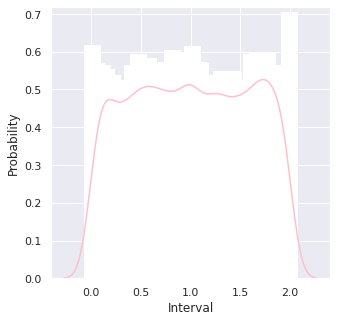
\includegraphics[scale=0.6]{assignment2.png}
    \caption{Distribution of $f_{(Y|X=1)}(y)$}
\end{figure}
From (0.0.4)
\begin{multline}
     E(Y|X=x)=\int_{-\infty}^{x-1}yf_{Y|X=x}(y)dy+\\ \int_{x-1}^{x+1}yf_{Y|X=x}(y)dy+\int_{x+1}^{\infty}yf_{Y|X=x}(y)dy
\end{multline}
\begin{align}
     E(Y|X=x)&=\int_{x-1}^{x+1}y\brak{\frac{1}{2}}dy\\
    &=x
\end{align}

\begin{align}
    E(Y)&=\int_{-\infty}^{\infty}E(Y|X=x)f_{X}(x)dx\\
    &=\int_{-\infty}^{\infty}xf_{X}(x)dx\\
    &=E(X)
\end{align}
From (0.0.3) we get 
\begin{align}
    E(Y)=1
\end{align}
\begin{align}
    Var(Y|X=x)&=\int_{-\infty}^{\infty}(y-E(Y))^2f_{Y|X=x}(y)dy\\
    &=\int_{x-1}^{x+1}(y-1)^2\brak{\frac{1}{2}}dy
\end{align}
\begin{align}
    Var(Y)&=\int_{-\infty}^{\infty}Var(Y|X=x)f_{X}(x)dx\\
    &=\brak{\frac{1}{2}}\int_{x-1}^{x+1}(y^2-2y+1)dy\\
    &=\brak{\frac{1}{2}}(\frac{6x^2+2}{3}+2-4x)\\
    &=x^2-2x+\frac{4}{3}
\end{align}

\begin{align}
    Var(Y)&=\int_{-\infty}^{\infty}(x^2-2x+\frac{4}{3})f_{X}(x)dx\\
    &=\int_{-\infty}^{\infty}x^2f_{X}(x)dx-2\int_{-\infty}^{\infty}xf_{X}(x)dx+\frac{4}{3}\int_{-\infty}^{\infty}f_{X}(x)dx
\end{align}
\begin{align}
  f_{X}(x)dx=1\\
 Var(X)=\int_{-\infty}^{\infty}x^2f_{X}(x)dx=\frac{5}{3}\\
 E(x)=\int_{-\infty}^{\infty}xf_{X}(x)dx=1\\
 \end{align}
 From (0.0.19), (0.0.20), (0.0.21) and (0.0.22) we get
 \begin{align}
     Var(Y)&=\frac{5}{3}-2+\frac{4}{3}\\
     &=1
 \end{align}
\textbf{$\therefore$ Option C is true}
\end{document}
\end{document}
